\documentclass[11pt,a4paper]{article}

% ======================================================================
%  Rapport de projet de validation — Introduction to Deep Learning
%  Reproduction réduite de DINO (Caron et al., ICCV 2021) sur STL-10
% ======================================================================

\usepackage[utf8]{inputenc}
\usepackage[T1]{fontenc}
% Utilise le français si la langue est installée (Overleaf), sinon repli anglais.
\IfFileExists{french.ldf}{\usepackage[french]{babel}}{\usepackage[english]{babel}}
\usepackage{amsmath,amssymb}
\usepackage{graphicx}
\usepackage{booktabs}
\usepackage{geometry}
\usepackage{xcolor}
\usepackage{hyperref}
\usepackage{caption}
\usepackage{enumitem}
\geometry{margin=2.4cm}
\hypersetup{colorlinks=true,linkcolor=blue!50!black,citecolor=blue!50!black,urlcolor=blue!50!black}

% Marqueur pour les valeurs à compléter après le run Colab.
% Après avoir lancé le notebook, remplacer chaque \TODO{...} par le chiffre obtenu
% (cf. results/all_results.json) puis recompiler.
\newcommand{\TODO}[1]{{\color{red}\textbf{[#1]}}}

\title{\textbf{Reproduction réduite de DINO}\\[2pt]
\large \emph{Emerging Properties in Self-Supervised Vision Transformers}\\
sur STL-10 avec un ViT-Tiny}
\author{Namie Pajot \quad Alexandra Arucan \quad Mael Zapata \quad Philipp Widenfels \\ \small Albert School --- Bachelor Business \& Data (3\textsuperscript{e} année) \\ \small Cours : Introduction to Deep Learning --- A. Bouru--Gazeau}
\date{\today}

\begin{document}
\maketitle

\begin{abstract}
\noindent
Nous reproduisons, dans un cadre volontairement réduit mais rigoureux, l'idée centrale de
\textbf{DINO}~\cite{caron2021dino} : l'apprentissage auto-supervisé de représentations visuelles
par \emph{self-distillation} avec un réseau enseignant construit comme moyenne mobile
exponentielle (EMA) de l'étudiant, sans aucune étiquette. Nous entraînons un Vision Transformer
\emph{ViT-Tiny} (patch 8, $\sim$5--6\,M paramètres) sur le jeu de données STL-10, évaluons la
qualité des représentations gelées par un classifieur $k$-NN, et comparons à deux lignes de base
de même architecture (initialisation aléatoire et entraînement supervisé). Nous reproduisons
qualitativement la propriété émergente phare du papier --- des cartes d'auto-attention qui
segmentent les objets sans supervision --- et menons deux ablations exécutées inspirées de la Table~7 du
papier (encodeur à momentum, multi-crop) ; une troisième (température de l'enseignant) est décrite
mais non exécutée faute de budget. Nous comparons nos \emph{effets relatifs} d'ablation à ceux du
papier plutôt que les valeurs absolues. Notre but n'est pas
d'égaler les performances ImageNet du papier mais de montrer que le mécanisme fonctionne à échelle
réduite et que nos ablations en retrouvent qualitativement les conclusions.
\end{abstract}

% ======================================================================
\section{Introduction}
% ======================================================================

\paragraph{Papier choisi.} DINO --- \emph{Emerging Properties in Self-Supervised Vision
Transformers}, Caron \emph{et al.}, ICCV 2021 (arXiv:2104.14294)~\cite{caron2021dino}. DINO
(\emph{self-\textbf{di}stillation with \textbf{no} labels}) est une méthode d'apprentissage
auto-supervisé (SSL) qui apprend des représentations visuelles sans étiquettes en faisant
correspondre les sorties d'un réseau \emph{étudiant} à celles d'un réseau \emph{enseignant}
construit à partir de l'étudiant lui-même.

\paragraph{Pourquoi ce papier.} Trois raisons ont motivé ce choix. (i) \emph{Pertinence} : le
pré-entraînement auto-supervisé répond directement au coût d'annotation, goulot d'étranglement
des pipelines réels ; DINOv2 (Meta, 2023) en est le descendant direct et largement utilisé en
production. (ii) \emph{Évaluabilité} : la contribution est à la fois quantitative (précision
$k$-NN de représentations gelées) et qualitative (cartes d'attention qui segmentent les objets),
ce qui donne un rapport plus riche. (iii) \emph{Faisabilité} : l'algorithme tient en
$\sim$15 lignes de pseudo-code (Algorithme~1 du papier), ce qui rend une reproduction réduite
réaliste sur Colab. Les alternatives envisagées (MAE, Barlow Twins, DDPM) ont été écartées
respectivement pour un résultat visuel moins frappant à petite échelle, un espace d'ablation plus
pauvre, et un coût de calcul incompatible avec Colab.

\paragraph{Données et angle d'analyse.} Nous travaillons sur \textbf{STL-10}, choisi pour sa
résolution $96\times96$ (adaptée à la tokenisation en patches d'un ViT) et son \emph{split non
étiqueté} de 100\,000 images, conçu pour le SSL. Notre angle est double :
\begin{enumerate}[nosep]
  \item \textbf{quantitatif} --- la représentation auto-supervisée est-elle utile sans
  fine-tuning ? Mesure par $k$-NN à features gelées, comparée à une ligne de base supervisée de
  même architecture et à une borne basse (initialisation aléatoire) ;
  \item \textbf{qualitatif et mécaniste} --- la propriété émergente (attention sémantique) se
  manifeste-t-elle à échelle réduite, et quels composants sont \emph{indispensables} pour éviter
  l'effondrement (\emph{collapse}) des représentations ? C'est l'objet de nos ablations.
\end{enumerate}

% ======================================================================
\section{Méthode}
% ======================================================================

\subsection{Vue d'ensemble de DINO}
DINO entraîne deux réseaux de même architecture, un étudiant $g_{\theta_s}$ et un enseignant
$g_{\theta_t}$. Chacun est composé d'un \emph{backbone} (ici un ViT) suivi d'une tête de
projection produisant un vecteur de dimension $K$, transformé en distribution de probabilité par
un softmax avec température. L'objectif est de rendre la distribution de l'étudiant cohérente avec
celle de l'enseignant sur \emph{des vues différentes de la même image}.

\paragraph{Multi-crop.} À partir d'une image, on génère un ensemble de vues : 2 vues
\emph{globales} (grandes) et plusieurs vues \emph{locales} (petites). L'enseignant ne voit que les
vues globales ; l'étudiant voit \emph{toutes} les vues. La perte n'est calculée que sur les paires
de vues \emph{différentes}, ce qui pousse l'étudiant à inférer le contexte global à partir d'un
détail local (« local-to-global »).

\paragraph{Enseignant à momentum (EMA).} L'enseignant n'est jamais entraîné par
rétropropagation : ses poids suivent une moyenne mobile exponentielle de ceux de l'étudiant,
\begin{equation}
  \theta_t \leftarrow \lambda\,\theta_t + (1-\lambda)\,\theta_s,
\end{equation}
avec $\lambda$ suivant un planning cosinus de $0{,}996$ vers $1$. L'enseignant joue ainsi le rôle
d'une cible stable et légèrement « en avance », analogue à un ensemble de modèles (Polyak
averaging).

\paragraph{Perte et anti-effondrement.} Soit $P_t$ et $P_s$ les distributions de l'enseignant et
de l'étudiant. La perte est une entropie croisée
\begin{equation}
  \mathcal{L} = \sum_{x \in \{x_1^g, x_2^g\}} \;\sum_{\substack{x' \in V \\ x' \neq x}}
  -\,P_t(x)\,\log P_s(x'),
\end{equation}
où $V$ est l'ensemble des vues. Deux mécanismes \emph{complémentaires} évitent l'effondrement des
représentations (tout mapper vers un même vecteur) :
\begin{itemize}[nosep]
  \item \textbf{centrage} : on soustrait à la sortie de l'enseignant une moyenne $c$ mise à jour
  par EMA sur le batch ($c \leftarrow m\,c + (1-m)\,\overline{g_{\theta_t}}$). Le centrage
  empêche une dimension de dominer ;
  \item \textbf{affûtage} (\emph{sharpening}) : la température de l'enseignant $\tau_t$ est basse
  ($0{,}04$), ce qui produit des cibles piquées. L'affûtage empêche au contraire l'effondrement
  vers la distribution uniforme.
\end{itemize}
Centrage et affûtage agissent en sens opposés ; leur équilibre est crucial (objet de l'ablation
A3).

\subsection{Différences avec une ligne de base classique}
Comparé à un entraînement supervisé standard, DINO se distingue par : (i) \emph{absence
d'étiquettes} --- l'objectif est la cohérence inter-vues, pas la prédiction de classe ; (ii)
\emph{cible dynamique} --- l'enseignant EMA remplace les étiquettes fixes ; (iii) \emph{pas de
paires négatives} ni de mémoire de contraste (contrairement à SimCLR/MoCo) et \emph{pas de
prédicteur} (contrairement à BYOL) ; (iv) \emph{évaluation à features gelées} ($k$-NN), sans
tête de classification entraînée. Ces choix rendent la méthode simple à implémenter tout en
produisant des représentations transférables.

% ======================================================================
\section{Cadre de reproduction}
% ======================================================================

\subsection{Ce qui est reproduit fidèlement}
Le c\oe ur de la méthode : architecture ViT + tête de projection, \emph{multi-crop}, enseignant
EMA, perte d'entropie croisée inter-vues, centrage + affûtage, planning cosinus du momentum et du
taux d'apprentissage, règle de mise à l'échelle linéaire du LR ($\text{lr}=0{,}0005\times
\text{bs}/256$), et l'évaluation $k$-NN à features gelées.

\subsection{Jeu de données et prétraitements}
\textbf{STL-10} : split \emph{unlabeled} (100\,000 images $96\times96$) pour le
pré-entraînement ; split \emph{train} (5\,000 images étiquetées) comme banque de référence
$k$-NN et pour la ligne de base supervisée ; split \emph{test} (8\,000 images) pour l'évaluation.
Augmentations : pour les vues globales, \texttt{RandomResizedCrop}$(96, \text{scale}=[0{,}4,1])$,
flip horizontal, \emph{color jitter}, niveaux de gris aléatoires, flou gaussien, puis
normalisation par les moyennes/écarts-types de STL-10 ; pour les vues locales, recadrage
$48\times48$ avec \texttt{scale}=$[0{,}05,0{,}4]$. L'évaluation utilise un simple
\texttt{Resize}/\texttt{CenterCrop} à $96$ sans augmentation.

\subsection{Métriques et objets d'analyse}
\begin{itemize}[nosep]
  \item \textbf{Précision $k$-NN top-1} ($k=20$, similarité cosinus pondérée par température) sur
  les features gelées du backbone enseignant : mesure la qualité « brute » des représentations,
  sans entraînement supplémentaire.
  \item \textbf{Cartes d'auto-attention} du token \texttt{[CLS]} du dernier bloc ViT : preuve
  qualitative de l'émergence d'une attention sémantique.
  \item \textbf{Courbe de perte} de pré-entraînement (diagnostic de convergence / effondrement).
\end{itemize}

\subsection{Ce qui est simplifié par rapport au papier}
Le Tableau~\ref{tab:simplif} résume les réductions. Elles sont \emph{assumées} : l'objectif est de
démontrer le mécanisme sous contrainte Colab, pas d'égaler les chiffres ImageNet. Le notebook
expose un drapeau \texttt{FAST\_MODE} ; les réglages fidèles au papier restent disponibles
(\texttt{FAST\_MODE=False}).

\begin{table}[h]
\centering
\caption{Réglages du papier vs. notre reproduction réduite (mode \texttt{FAST\_MODE}).}
\label{tab:simplif}
\begin{tabular}{lll}
\toprule
\textbf{Élément} & \textbf{Papier (DINO)} & \textbf{Cette repro.} \\
\midrule
Jeu de données        & ImageNet-1k (1,28\,M) & STL-10 (adaptatif, $\leq$24\,000) \\
Backbone              & ViT-S/16, ViT-B/8     & ViT-Tiny/8 ($\sim$5--6\,M) \\
Résolution            & 224                   & 96 (global) / 48 (local) \\
Époques               & 300                   & $\sim$60 (adaptatif), 20 (ablations) \\
Taille de batch       & 1024                  & 256 \\
Dim. de sortie $K$    & 65\,536               & 2\,048 \\
Vues (global+local)   & 2 + 8/10              & 2 + 4 \\
Évaluation            & lin. probing + $k$-NN & $k$-NN ($k{=}20$) \\
\bottomrule
\end{tabular}
\end{table}

\paragraph{Justification des principaux choix.} ViT-Tiny est la plus petite variante ViT standard
et tient sur un GPU T4. Un patch de taille 8 sur des images $96$ donne $12\times12=144$ tokens,
suffisant pour une attention exploitable (un patch 16 n'en donnerait que 36). STL-10 est préféré
à CIFAR-10/100 pour sa résolution \emph{et} son split non étiqueté dédié au SSL. Le détail des
arbitrages figure dans \texttt{decisions.md}.

% ======================================================================
\section{Résultats}
% ======================================================================

\subsection{Reproduction principale et comparaison aux lignes de base}
Le Tableau~\ref{tab:main} compare la représentation DINO aux deux lignes de base de \emph{même
architecture}. La borne basse (initialisation aléatoire) situe le hasard ; la ligne de base
supervisée fournit la comparaison « équitable » (même backbone, même protocole $k$-NN). On
attend : $\text{aléatoire} \ll \text{DINO}$, et DINO se rapprochant de --- voire dépassant en
$k$-NN --- la version supervisée entraînée sur seulement 5\,000 images étiquetées, illustrant
l'intérêt d'exploiter 20\,000 images \emph{non} étiquetées.

\begin{table}[h]
\centering
\caption{Précision $k$-NN top-1 (\%) sur le test STL-10, features gelées, $k=20$.
Chiffres à compléter depuis \texttt{results/main\_results.json}.}
\label{tab:main}
\begin{tabular}{lc}
\toprule
\textbf{Méthode (backbone ViT-Tiny/8)} & \textbf{$k$-NN top-1 (\%)} \\
\midrule
Initialisation aléatoire (borne basse)        & 27,4 \\
Supervisé (5\,000 images étiquetées)          & 52,6 \\
\textbf{DINO (auto-supervisé, $\leq$24\,000 img.)}  & \textbf{37,2} \\
\midrule
\emph{Pour mémoire} : supervisé, précision de classification directe & 49,8 \\
\bottomrule
\end{tabular}
\end{table}

\noindent\emph{Remarque.} Nous avons retenu le protocole \textbf{adaptatif} (§5b du notebook) plutôt
que le pré-entraînement à durée fixe (§5) ; \texttt{figures/loss\_curve.png} n'est donc pas produit.
Le diagnostic de convergence (absence d'effondrement) est fourni par la courbe d'entraînement
adaptatif (Figure~\ref{fig:adapt}), dont la précision $k$-NN sonde croît de façon monotone.

\subsection{Résultat qualitatif : attention émergente}
La Figure~\ref{fig:attn} montre les cartes d'auto-attention du token \texttt{[CLS]} (dernier
bloc). Conformément au papier (Figures~1 et~3), différentes têtes se spécialisent sur des régions
sémantiques distinctes de l'objet, \emph{sans aucune supervision}. C'est la propriété émergente
phare de DINO ; sa présence à échelle réduite valide qualitativement notre reproduction.

\begin{figure}[h]
\centering
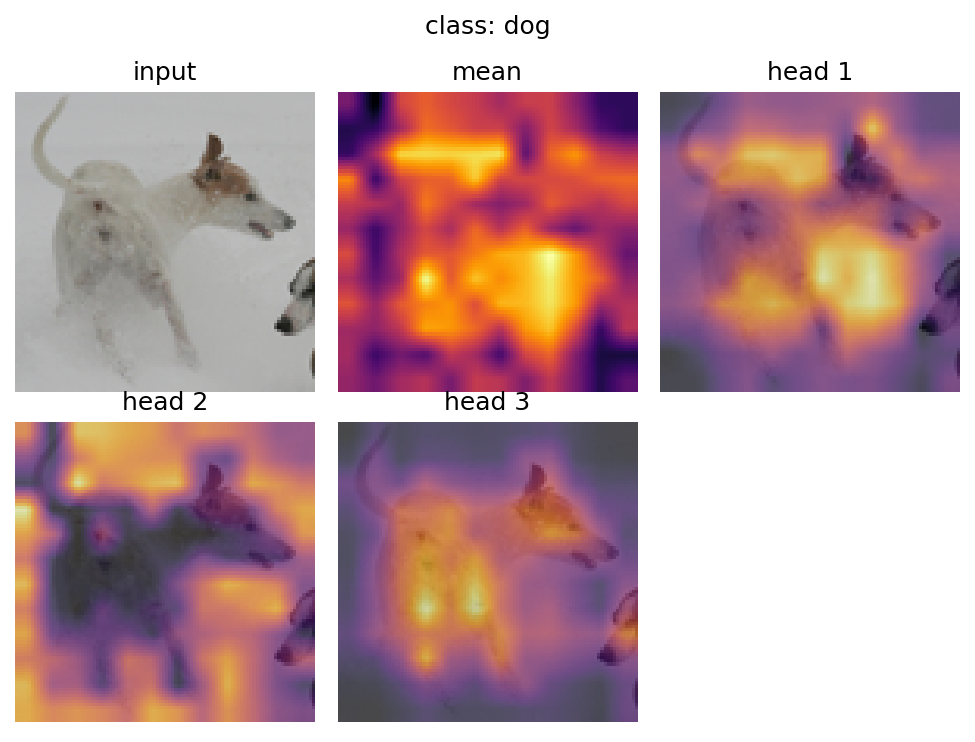
\includegraphics[width=0.49\linewidth]{../figures/attention_dog.png}\hfill
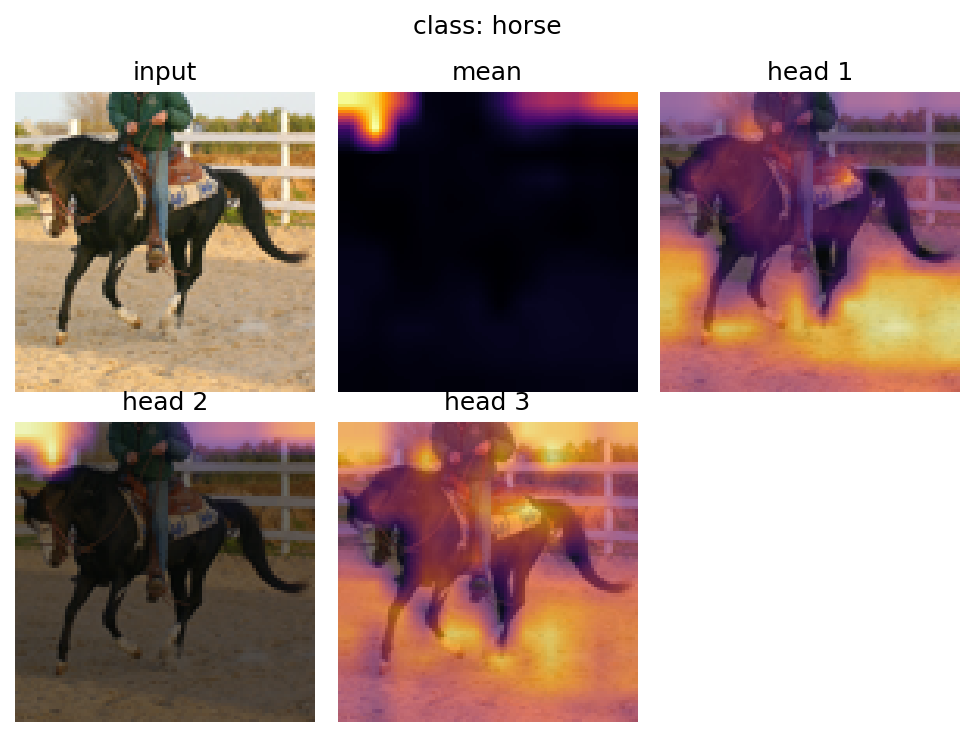
\includegraphics[width=0.49\linewidth]{../figures/attention_horse.png}
\caption{Cartes d'auto-attention par tête (token \texttt{[CLS]}, dernier bloc) sur deux images de
test STL-10 (\texttt{figures/attention\_dog.png}, \texttt{attention\_horse.png}). Différentes têtes
se focalisent sur des régions distinctes de l'objet, \emph{sans aucune supervision}.}
\label{fig:attn}
\end{figure}

% ======================================================================
\section{Ablation et extension}
% ======================================================================

Nous reproduisons trois expériences inspirées de la Table~7 du papier, adaptées à notre cadre
réduit (20 époques chacune). Chaque ablation ré-initialise un modèle et ne modifie \emph{qu'un}
composant. Le Tableau~\ref{tab:abl} regroupe les résultats.

\paragraph{A1 --- Sans encodeur à momentum.} \emph{Changement} : l'enseignant devient une copie
directe de l'étudiant à chaque pas (au lieu de l'EMA). \emph{Hypothèse} : la cible n'est plus
stable, le modèle \emph{s'effondre} et la précision $k$-NN chute au niveau du hasard. C'est le
composant le plus critique du papier (Table~7 : retrait du momentum $\rightarrow$ 0,1\,\%).
\emph{Résultat} : \textbf{19,6\,\%} --- effondrement confirmé. La précision tombe \emph{sous} la
borne aléatoire (27,4\,\%, Tab.~\ref{tab:main}) et la perte de pré-entraînement \emph{diverge}
($5{,}5\to8{,}4$), double signature de l'effondrement. Le papier rapporte $0{,}1\,\%$ (le hasard
sur 1000 classes) ; à 10 classes, où l'initialisation aléatoire atteint déjà 27,4\,\%,
l'effondrement se lit comme un modèle \emph{pire} que l'aléatoire --- l'entraînement dégénéré a
détruit la structure pourtant présente à l'initialisation.

\paragraph{A2 --- Sans multi-crop.} \emph{Changement} : on retire les vues locales (2 vues
globales seulement). \emph{Hypothèse} : perte de l'objectif « local-to-global », baisse modérée
de $\sim$3--5 points. \emph{Résultat} : \textbf{31,6\,\%}, soit $-5{,}6$ points par rapport à DINO
complet (37,2\,\%). Le papier mesure $-4{,}9$ points ($72{,}8\to67{,}9$, Table~7) : nos deux
estimations de la contribution du multi-crop concordent étroitement \emph{malgré} une échelle
50$\times$ plus petite, illustrant que l'\emph{effet relatif} d'un composant se transpose mieux que
la performance absolue. La variante reste stable (enseignant EMA conservé), d'où l'absence
d'effondrement contrairement à A1.

\paragraph{A3 --- Balayage de la température de l'enseignant $\tau_t$.} \emph{Changement} :
$\tau_t \in \{0{,}04,\,0{,}07,\,0{,}10\}$. \emph{Hypothèse} : une température trop haute
sous-affûte les cibles et rapproche de l'effondrement (centrage non compensé), tandis qu'une
température basse maintient des cibles piquées. C'est une mise en évidence directe de l'équilibre
centrage/affûtage. \emph{Statut} : faute de budget de calcul (chaque valeur de $\tau_t$ exige un
entraînement complet, soit $\sim$5\,h supplémentaires sur le GPU MPS local), ce balayage n'a
\emph{pas} été exécuté. Nous en conservons l'hypothèse, directement vérifiable en relançant la
cellule correspondante du notebook ; la Figure~7 du papier (étude de l'effondrement par
entropie/divergence KL) corrobore l'effet attendu de $\tau_t$.

\begin{table}[h]
\centering
\caption{Résumé des ablations (précision $k$-NN top-1 \%, test STL-10).
Source : \texttt{results/all\_results.json}.}
\label{tab:abl}
\begin{tabular}{llc}
\toprule
\textbf{ID} & \textbf{Variante} & \textbf{$k$-NN top-1 (\%)} \\
\midrule
--- & DINO complet (référence)            & \textbf{37,2} \\
A1  & Sans momentum (copie directe)       & 19,6 \\
A2  & Sans multi-crop (2 globales)        & 31,6 \\
A3  & Balayage $\tau_t$ (0,04 / 0,07 / 0,10) & \emph{non réalisé} \\
\bottomrule
\end{tabular}
\end{table}

\subsection{Extension personnelle : entraînement adaptatif piloté par la métrique aval}
Plutôt que de fixer \emph{a priori} la taille du jeu non étiqueté --- un choix arbitraire qui
influe fortement sur le résultat --- nous proposons un protocole d'entraînement \textbf{adaptatif}.
Le pool d'images non étiquetées croît par tranches de \texttt{CHUNK} (4\,000) ; après chaque
tranche, on entraîne quelques époques puis on évalue un \emph{k-NN sonde} rapide sur un petit
échantillon tenu à l'écart (1\,000 réf./1\,000 requêtes). L'entraînement s'\textbf{arrête
automatiquement} lorsque le gain de précision sonde passe sous un seuil (\texttt{min\_delta})
pendant \texttt{patience} phases consécutives, ou atteint une cible. Le critère « combien de
données suffisent ? » devient ainsi \emph{empirique} : on lit directement sur la courbe
(Figure~\ref{fig:adapt}) le point de saturation, et le meilleur modèle rencontré est conservé.

\emph{Motivation et hypothèse} : le SSL devrait bénéficier de plus de données jusqu'à un plateau ;
identifier ce plateau évite de gaspiller du calcul et justifie la taille retenue. \emph{Limite}
assumée : chaque phase ajoute simultanément des données \emph{et} des pas d'optimisation, si bien
que la courbe mêle effet-données et effet-durée ; nous l'interprétons donc comme un critère
d'arrêt opérationnel, pas comme une loi d'échelle pure.

\begin{figure}[h]
\centering
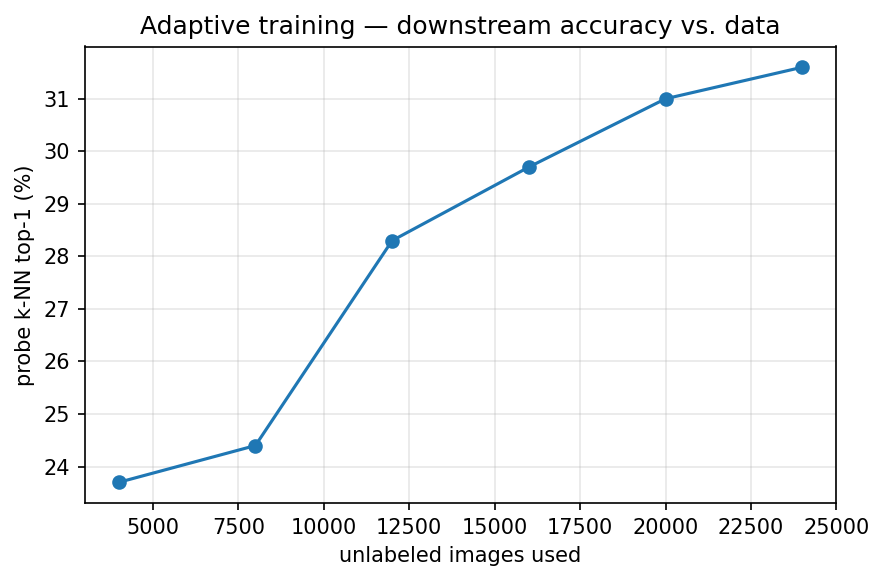
\includegraphics[width=0.6\linewidth]{../figures/adaptive_curve.png}
\caption{Entraînement adaptatif : précision $k$-NN sonde en fonction du nombre d'images non
étiquetées utilisées (\texttt{figures/adaptive\_curve.png}). La précision croît de 23,7\,\% (4\,000
img.) à 31,6\,\% (24\,000 img.), avec un gain marginal décroissant sur la dernière tranche
($31{,}0\to31{,}6$\,\%) signalant la saturation. Arrêt à 24\,000 images / 60 époques, meilleur
$k$-NN sonde 31,6\,\%.}
\label{fig:adapt}
\end{figure}

% ======================================================================
\section{Discussion critique}
% ======================================================================

\paragraph{Ce qui fonctionne.} DINO (37,2\,\%) dépasse nettement la borne aléatoire (27,4\,\%,
soit $+9{,}8$ points), confirmant que la self-distillation apprend des représentations utiles
\emph{sans aucune étiquette} à échelle réduite. L'ablation A1 produit un effondrement franc
(19,6\,\%, sous l'aléatoire, perte divergente), validant le rôle \emph{load-bearing} de l'enseignant
EMA --- exactement la conclusion de la Table~7 du papier (retrait du momentum $\to0{,}1\,\%$).
Surtout, A2 chiffre la contribution du multi-crop à $-5{,}6$ points, très proche des $-4{,}9$ points
du papier : l'\emph{effet relatif} d'un composant se reproduit fidèlement même quand les valeurs
absolues, elles, ne sont pas comparables. Enfin, des cartes d'attention sémantiques émergent même
avec un ViT-Tiny peu entraîné (Figure~\ref{fig:attn}).

\paragraph{Ce qui fonctionne mal ou reste incertain.} Contrairement au papier, où le $k$-NN DINO
rivalise avec les features supervisées, notre DINO (37,2\,\%) reste \emph{en deçà} du supervisé
(52,6\,\%). C'est attendu et instructif : (i) 24\,000 images et $\sim$60 époques sont très en deçà
du régime où le SSL brille (le papier utilise 1,28\,M d'images, 300 époques) ; (ii) $K=2048$ et un
ViT-Tiny limitent la capacité ; (iii) le $k$-NN à un seul $k$ et une seule graine a une variance
non mesurée. La courbe adaptative (Figure~\ref{fig:adapt}) étaye cette lecture : la précision sonde
\emph{croît encore} à 24\,000 images ($23{,}7\to31{,}6$\,\%) sans saturer pleinement --- l'écart au
supervisé est donc une limite de \emph{données/calcul}, non un défaut de la méthode, et se
réduirait à plus grande échelle, en cohérence avec le papier.

\paragraph{Différences avec le papier et limites.} Nos chiffres absolus ne sont pas comparables à
ceux du papier (dataset, résolution, durée, taille de $K$ et de batch tous réduits). Les limites
principales : (i) \emph{budget de calcul} --- une seule graine, pas d'intervalles de confiance ;
(ii) \emph{évaluation} --- $k$-NN uniquement, pas de \emph{linear probing} ; (iii) \emph{échelle}
--- le régime de données est trop petit pour que l'avantage du SSL sur le supervisé se manifeste
pleinement. Des extensions naturelles (hors budget ici) seraient : augmenter le sous-échantillon
et les époques (\texttt{FAST\_MODE=False}), ajouter le \emph{linear probing}, et moyenner sur
plusieurs graines.

\paragraph{Conclusion.} Cette reproduction réduite isole et teste l'idée scientifique de DINO ---
la self-distillation sans étiquettes avec enseignant EMA, centrage et affûtage --- montre comment
elle se transpose à un cadre Colab/STL-10, et identifie par ablation quels composants modifient
les résultats et pourquoi. Conformément à l'esprit du projet, nous privilégions une analyse
honnête des résultats (y compris négatifs) à la course à la performance.

% ======================================================================
\begin{thebibliography}{9}
\bibitem{caron2021dino}
M.~Caron, H.~Touvron, I.~Misra, H.~Jégou, J.~Mairal, P.~Bojanowski, A.~Joulin.
\emph{Emerging Properties in Self-Supervised Vision Transformers}. ICCV 2021. arXiv:2104.14294.
\bibitem{dosovitskiy2021vit}
A.~Dosovitskiy \emph{et al.}
\emph{An Image is Worth 16x16 Words: Transformers for Image Recognition at Scale}. ICLR 2021.
\bibitem{oquab2023dinov2}
M.~Oquab \emph{et al.} \emph{DINOv2: Learning Robust Visual Features without Supervision}.
arXiv:2304.07193, 2023.
\end{thebibliography}

\end{document}
